% Maybe generalize the preference sheet. this was somewhat considered with the server as well.

\subsection{Library}
As none of the group members had any previous experience with image processing, it was quite unrealistic to try to implement all of the image processing techniques needed for this project, and at the same time make them optimized enough, so it could work well and fast on a Raspberry Pi computer with its limited resources. For this reason the group decided to use an existing image processing library to ease the implementation process. After some research and experiments, we decided to go with one of the most popular and well documented libraries called OpenCV\footnote{OpenCV homepage: \url{http://opencv.org/}.}. OpenCV is an open source computer vision and machine learning software library that has more than 500~\cite{opencv_1} optimized algorithms for image processing. Furthermore, it provides interfaces to multiple popular programming languages, including C\texttt{++}, C, Python and Java.

\subsection{Programming Language}
For determining which programming language to use for image processing on Raspberry Pi computers, a skill and preference document (Appendix~\ref{sec:Skill_Preference_Sheet}) was created, where both ITU and Strathmore University teams indicated their skill and preference for various programming languages. The two languages that stood out the most were Java and Python, thus to choose one of them, we decided to benchmark\footnote{Code used for benchmarks: Java - \url{http://itu.dk/people/tmis/javatest/}, Python - \url{http://itu.dk/people/tmis/pytest/}.} them in order to compare their performance. The results are presented in the next section.

\subsubsection{Performance Comparison Between Java and Python}
Since the project dealt with a real-time vision application that had to process large amount of frames, we were interested in how fast Java and Python can perform different image processing algorithms. Benchmarks were performed on a laptop\footnote{Toshiba Satellite L855 Laptop (Intel Core i7-3630QM 2.40 GHZ, 4GB DDR3 1600MHz, Radeon HD7670M 2GB, Windows 7 OS).} and a Raspberry Pi computer\footnote{Raspberry Pi Computer (ARM1176JZF-S 700MHz, 512 MB memory, Broadcom VideoCore IV graphics, Linux Raspbian OS).} to give some perspective on how much faster a modern laptop is compared to a Raspberry Pi computer.

\begin{itemize}
\item At first we tried to benchmark how fast can Java and Python perform a simple matrix multiplication of two $300 \times 300$ size matrices. The results are illustrated in Figure~\ref{fig:benchmark_multiplication}. We can clearly see that Java was way faster than Python in this benchmark. It took Java less than half of a second to perform the multiplication of two $300 \times 300$ size matrices on a laptop, whereas it took more than 3 seconds to do the same in Python (Figure~\ref{fig:benchmark_1}). Multiplication on a Raspberry Pi computer (Figure~\ref{fig:benchmark_2}) was naturally much slower than on a laptop. Java was again much faster than it's counterpart by dealing with the task in less than 23 seconds, whereas Python was very close to hitting 2 minute mark to accomplish the same task.

In conclusion as it was expected - Java convincingly won the first benchmark.

\begin{figure}[htb]
		\centering
		\subfigure[Average time (in seconds) needed to multiply two $300 \times 300$ size matrices in Java and Python on a laptop]{
		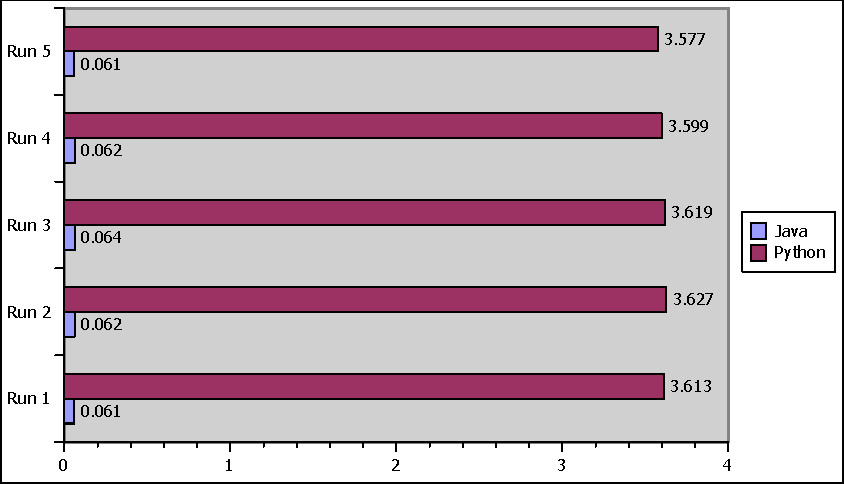
\includegraphics[scale=0.95]{benchmark/benchmark_1}
		\label{fig:benchmark_1}}
		\quad
		\subfigure[Average time (in seconds) needed to multiply two $300 \times 300$ size matrices in Java and Python on a Raspberry Pi computer]{
		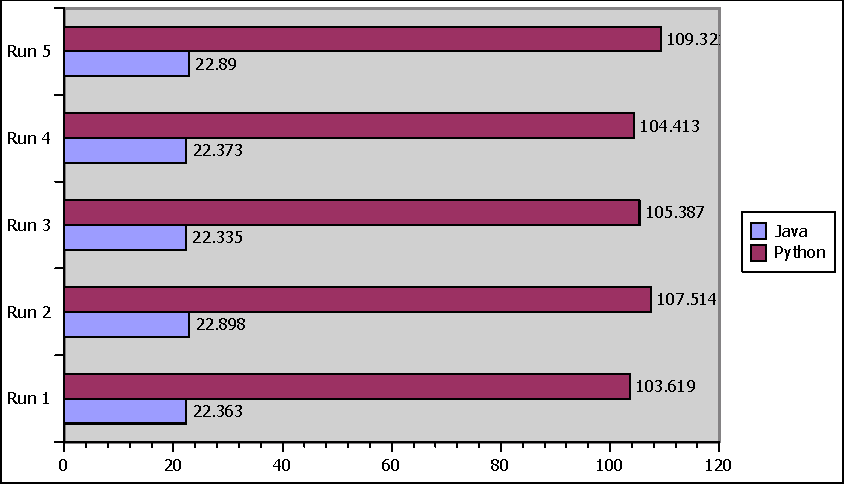
\includegraphics[scale=0.95]{benchmark/benchmark_2}
		\label{fig:benchmark_2}}
		\caption{Benchmark of matrix multiplication of two $300 \times 300$ size matrices}
		\label{fig:benchmark_multiplication}
\end{figure}

\item The second benchmark involved testing how fast Java and Python can perform different image processing algorithms. For this benchmark we used the OpenCV library that we introduced earlier. OpenCV has Java and Python interfaces and all the computations are performed on the native level\footnote{In C\texttt{++}.}, hence we have some overhead from the language bindings of the API calls. Consequently, the purpose of this benchmark was to see, which language - Java or Python - has less overhead and can perform API calls faster. 

As we can see in Figure~\ref{fig:benchmark_image_processing}, the difference between Java and Python in this benchmark was rather small on both, laptop~\ref{fig:benchmark_3} and Raspberry Pi computer~\ref{fig:benchmark_4}. This was rather surprising at first, since Java had a big edge in the first benchmark. One can speculate that Python's interface to OpenCV library has been implemented in a more efficient way than Java's, thus the outcome. In general, the difference was only in terms of a few milliseconds, however, it was a good enough reason for us to choose Python's interface to OpenCV library for image processing part in this project.

Overall, the group was happy with the choice of the Python programming language for the image processing part, as it was rather easy to build complicated structures with only a few lines of code.

\begin{figure}[htb]
	\centering
	\subfigure[Average time (in seconds) needed to process images in Java and Python on a laptop]{
	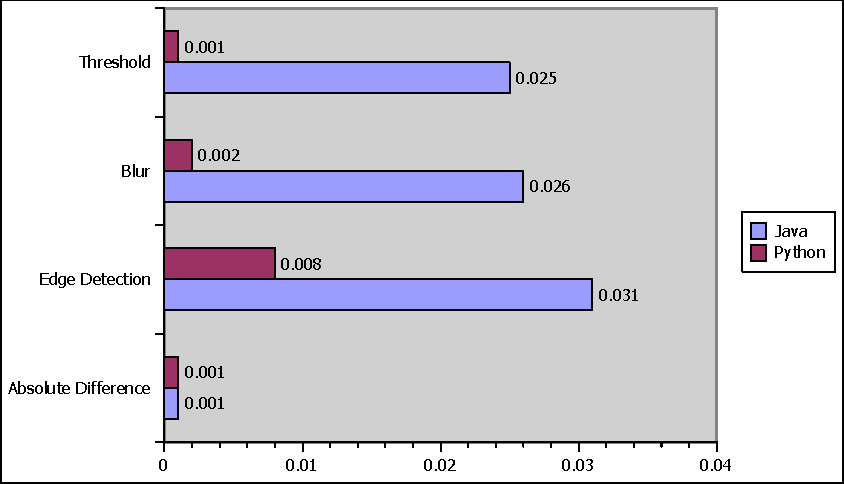
\includegraphics[scale=0.95]{benchmark/benchmark_3}
	\label{fig:benchmark_3}}
	\quad
	\subfigure[Average time (in seconds) needed to process images in Java and Python on a Raspberry Pi computer]{
	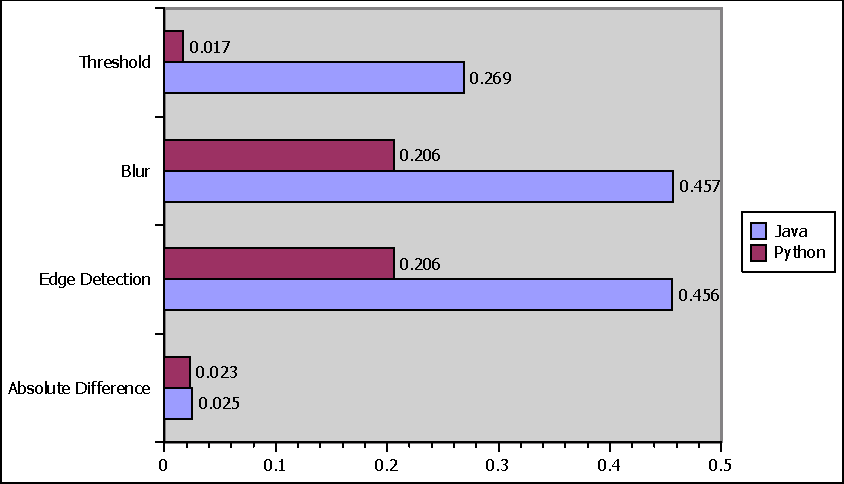
\includegraphics[scale=0.95]{benchmark/benchmark_4}
	\label{fig:benchmark_4}}
	\caption{Benchmark of image processing}
	\label{fig:benchmark_image_processing}
\end{figure}
\end{itemize}